%! Author = breandan
%! Date = 3/7/20

% Preamble
\documentclass{beamer}

% Packages
\usepackage{amsmath}
\usepackage{graphicx}
\usepackage{sourcecodepro}
\usepackage{listings}
\usepackage{amsfonts}
\usepackage{tikz}
\usepackage{tikz-qtree}
\usepackage{amsthm}
\usepackage{bm}

%\theoremstyle{definition}
%\newtheorem{definition}{Definition}[section]

\mode<presentation> { \usetheme{Madrid} }

\title{Discriminative Embeddings}
\subtitle{of Latent Variable Models for Structured Data}
\author{Hanjun Dai, Bo Dai, Le Song}
\institute[McGill]{
    presentation by \\
    Breandan Considine \\
    McGill University \\
    \medskip
    \textit{breandan.considine@mail.mcgill.ca}
}
\date{\today}
% Document
\begin{document}

    \begin{frame}
        \titlepage
    \end{frame}

    \begin{frame}
        \frametitle{What is a kernel?}
        A feature map transforms the input space to a feature space:
        \begin{equation}
            \varphi: \overbrace{\mathbb R^n}^\text{Input space} \to \overbrace{\mathbb R^m}^\text{Feature space}
        \end{equation}
        Kernel functions generalize the notion of inner products to feature maps:
        \begin{equation}
            k(\mathbf x, \mathbf y) = \varphi(\mathbf x)^\intercal \varphi(\mathbf y)
        \end{equation}
        Gives us $\varphi(x)^\intercal\varphi(y)$ without directly computing $\varphi(x)$ or $\varphi(y)$
    \end{frame}

    \begin{frame}
        \frametitle{What is a kernel?}
        Consider the univariate polynomial regression algorithm:
        \begin{equation}
            \hat{f}(\mathbf x; \bm\beta) = \beta\varphi(\mathbf x)
            = \beta_0 + \beta_1 x + \beta_2 x^2 + \cdots + \beta_m x^m = \sum\limits_{j=0}^{m} \beta_j x^{j}
        \end{equation}
        Where $\varphi(\mathbf x) = [1, x_1, x_2^2, x_3^3, \ldots, x_m^m]$. We seek $\bm\beta$ minimizing the error:
        \begin{equation}
            \bm\beta^* = \underset{\bm\beta}{\operatorname{argmin}}||\mathbf Y - \hat{\mathbf f}(\mathbf X; \bm\beta)||^2
        \end{equation}
        We can solve for $\bm \beta^*$ using the normal equation or gradient descent:
        \begin{align}
            \bm\beta^* &= (\mathbf X^\intercal \mathbf X)^{-1}\mathbf X^\intercal\mathbf Y \\
            \bm\beta' &\leftarrow \bm\beta - \alpha \nabla_{\bm\beta}||\mathbf Y - \hat{\mathbf f}(\mathbf X; \bm\beta)||^2
        \end{align}
        What happens if we have a multivariate polynomial?
        \begin{equation}
            z(x, y) = 1 + \beta_{x} x + \beta_{y}y + \beta_{xy} xy + \beta_{x^2} x^2 + \beta_{y^2} y^2 + \beta_{xy^2} xy^2 + \ldots
        \end{equation}
    \end{frame}

    \begin{frame}
        \frametitle{What is a kernel?}
        Consider the polynomial kernel $k(\mathbf x, \mathbf y) = (1 + \mathbf x^T \mathbf y)^2$ with $\mathbf x, \mathbf y \in \mathbb R^2$.

        \begin{align}
            k(\mathbf x, \mathbf y) & = (1 + \mathbf x^T \mathbf y)^2 = (1 + x_1 \, y_1  + x_2 \, y_2)^2 \\
            & = 1 + x_1^2 y_1^2 + x_2^2 y_2^2 + 2 x_1 y_1 + 2 x_2 y_2 + 2 x_1 x_2 y_1 y_2 \
        \end{align}

        This gives us the same result as computing the 6 dimensional feature map:

        \begin{align}
            k(\mathbf x, \mathbf y) &= \varphi(\mathbf x)^\intercal \varphi(\mathbf y) \\
            &=[1, x_1^2, x_2^2, \sqrt{2} x_1, \sqrt{2} x_2, \sqrt{2} x_1 x_2]^\intercal\begin{bmatrix}1\\ y_1^2\\ y_2^2\\ \sqrt{2} y_1\\ \sqrt{2} y_2\\ \sqrt{2} y_1 y_2\end{bmatrix}
        \end{align}

        But does not require computing $\varphi(x)$ or $\varphi(y)$.
    \end{frame}

    \begin{frame}
        \frametitle{Examples of common kernels}
        \centering{Popular kernels}
            \begin{center}
                \begin{tabular}{|c|c|c|} \hline
                    Polynomial & $k(\mathbf{x},\mathbf{y}):=(\mathbf{x}^{T}\mathbf{y}+r)^{n}$ & $\quad \mathbf{x},\mathbf{y}\in \mathbb {R} ^{d}, n \in \mathbb N, r\geq 0$ \\ \hline
                    Laplacian & $k(\mathbf{x},\mathbf{y}):=exp\left(-\alpha \|\mathbf{x}-\mathbf{y}\|\right)$ & $\quad \mathbf{x},\mathbf{y}\in \mathbb {R} ^{d},\alpha >0$ \\ \hline
                    Gaussian RBF & $k(\mathbf {x}, \mathbf {y}):=\exp \left(-{\frac {\|\mathbf {x} -\mathbf {y} \|^{2}}{2\sigma ^{2}}}\right)$ & $\quad \mathbf{x},\mathbf{y}\in \mathbb {R} ^{d},\sigma >0$ \\ \hline
                \end{tabular}
            \end{center}

        \centering{Popular Graph Kernels}
        \begin{center}
            \begin{tabular}{|c|l|l|} \hline
            RW & $k_\times(G, H) := \sum\limits_{i, j = 1}^{|V_\times|}[\sum\limits_{n=1}^\infty\mathbf{\lambda}^{n}A^n_\times]_{ij} = \mathbf{e}^\intercal(\mathbf{I} - \lambda A_\times)^{-1}\mathbf{e}$ & $\mathcal O(n^6)$ \\\hline
            SP & $k_{SP}(G, H) := \sum\limits_{s_1\in SD(G)}\sum\limits_{s_2 \in SD(H)} k(s_1, s_2)$ & $\mathcal O(n^4)$ \\\hline
            WL & \begin{tabular}$l^{(i)}(G) :=$ \begin{cases}$\text{deg}_v, \forall v \in G$&$i = 1$\\$HASH(\{\{l^{(i-1)}(u), \forall u \in \mathcal{N}(v)\}\})$&$i > 1$\end{cases}\\$k_{WL}(G, H):=\langle\psi_{WL}(G), \psi_{WL}(H)\rangle$\end{tabular} & $\mathcal O(hm)$ \\\hline
            \end{tabular}
        \end{center}
        \tiny{\url{https://people.mpi-inf.mpg.de/~mehlhorn/ftp/genWLpaper.pdf}}
\end{frame}

\begin{frame}
        \frametitle{What is an inner product space?}
        Let $X$ be a vector space over the reals.
        \begin{definition}
            A function $f: X \rightarrow \mathbb R$ is \textbf{linear} iff $f(\alpha x)= \alpha f(x)$
            and $f(x+z)=f(x)+f(z)$ for all $\alpha\in\mathbb R, x,z \in X$.
        \end{definition}

        \begin{definition}
            $X$ is an \textbf{inner product space} if there exists a symmetric bilinear map $\langle \cdot ,\cdot \rangle :X\times X\to \mathbb R$ if $\forall \mathbf x \in X, \langle \mathbf x,\mathbf x \rangle > 0$ (i.e. is positive definite).
        \end{definition}
        \begin{center}
            \begin{tabular}{ c c c }
                \textbf{Scalar Product} & \textbf{Vector Dot Product} & \textbf{Random Variable} \\
                $\langle x,y\rangle := xy$ &
                $\left\langle {\begin{bmatrix}x_{1}\\\vdots \\x_{n}\end{bmatrix}},{\begin{bmatrix}y_{1}\\\vdots \\y_{n}\end{bmatrix}}\right\rangle :=x^{\textsf {T}}y$ &
                $\langle X,Y\rangle :=\operatorname {E} (XY)$
            \end{tabular}
        \end{center}
    \end{frame}

    \begin{frame}
        \frametitle{What is a Hilbert space?}
            Let $d: X\times X \rightarrow \mathbb R^{\geq 0}$ be a metric on the space $X$. \\
        \begin{block}{Definition: Cauchy sequence}
            A sequence $\{x_n\}$ is called a \textbf{Cauchy sequence} if $\forall \varepsilon > 0, \exists N \in \mathbb{N}, \text{ such that } \forall n,m \geq N, d(x_n,x_m)\leq \varepsilon$. \\
        \end{block}
        \begin{block}{Definition: Completeness}
            $X$ is called \textbf{complete} if every Cauchy sequence converges to a point in $X$.
        \end{block}
        \begin{block}{Definition: Separability}
            $X$ is called \textbf{separable} if there exists a sequence $\{x_n\}_{n = 1}^\infty \in X$ s.t. every nonempty open subset of $X$ contains at least one element of the sequence.
        \end{block}
        \begin{block}{Definition: Hilbert space}
            A Hilbert space $\mathcal H$ is an inner product space that is complete and separable.
        \end{block}
    \end{frame}

    \begin{frame}
        \frametitle{Properties of Hilbert Spaces}
        \begin{block}{Hilbert space inner products are kernels}
            The inner product $\langle\cdot ,\cdot \rangle_{\mathcal H}:\mathcal H\times \mathcal H\to \mathbb {R}$ is a PD positive definite kernel:
            $\sum\limits_{i,j=1}^{n}c_{i}c_{j}(x_{i},x_{j})_{\mathcal H}=\left(\sum _{i=1}^{n}c_{i}x_{i},\sum\limits_{j=1}^{n}c_{j}x_{j}\right)_{\mathcal H}=\left\|\sum \limits_{i=1}^{n}c_{i}x_{i}\right\|_{\mathcal H}^{2}\geq 0$
        \end{block}

        \begin{block}{Reproducing Kernel Hilbert Space (RKHS)}
            Any continuous, symmetric, positive definite kernel $k: X \times X\rightarrow \mathbb R$ has a corresponding Hilbert space, which induces a feature map $\varphi: X \rightarrow \mathcal H$ satisfying $k(x,y) = \langle\varphi(x),\varphi(y)\rangle $_{\mathcal H}.
        \end{block}

        \tiny{\url{http://jmlr.csail.mit.edu/papers/volume11/vishwanathan10a/vishwanathan10a.pdf}}
    \end{frame}

    \begin{frame}
        \frametitle{Structured data kernels}
    \end{frame}

    \begin{frame}
        \frametitle{Belief propagation}
    \end{frame}

    \begin{frame}
        \frametitle{Results}
        \begin{center}
        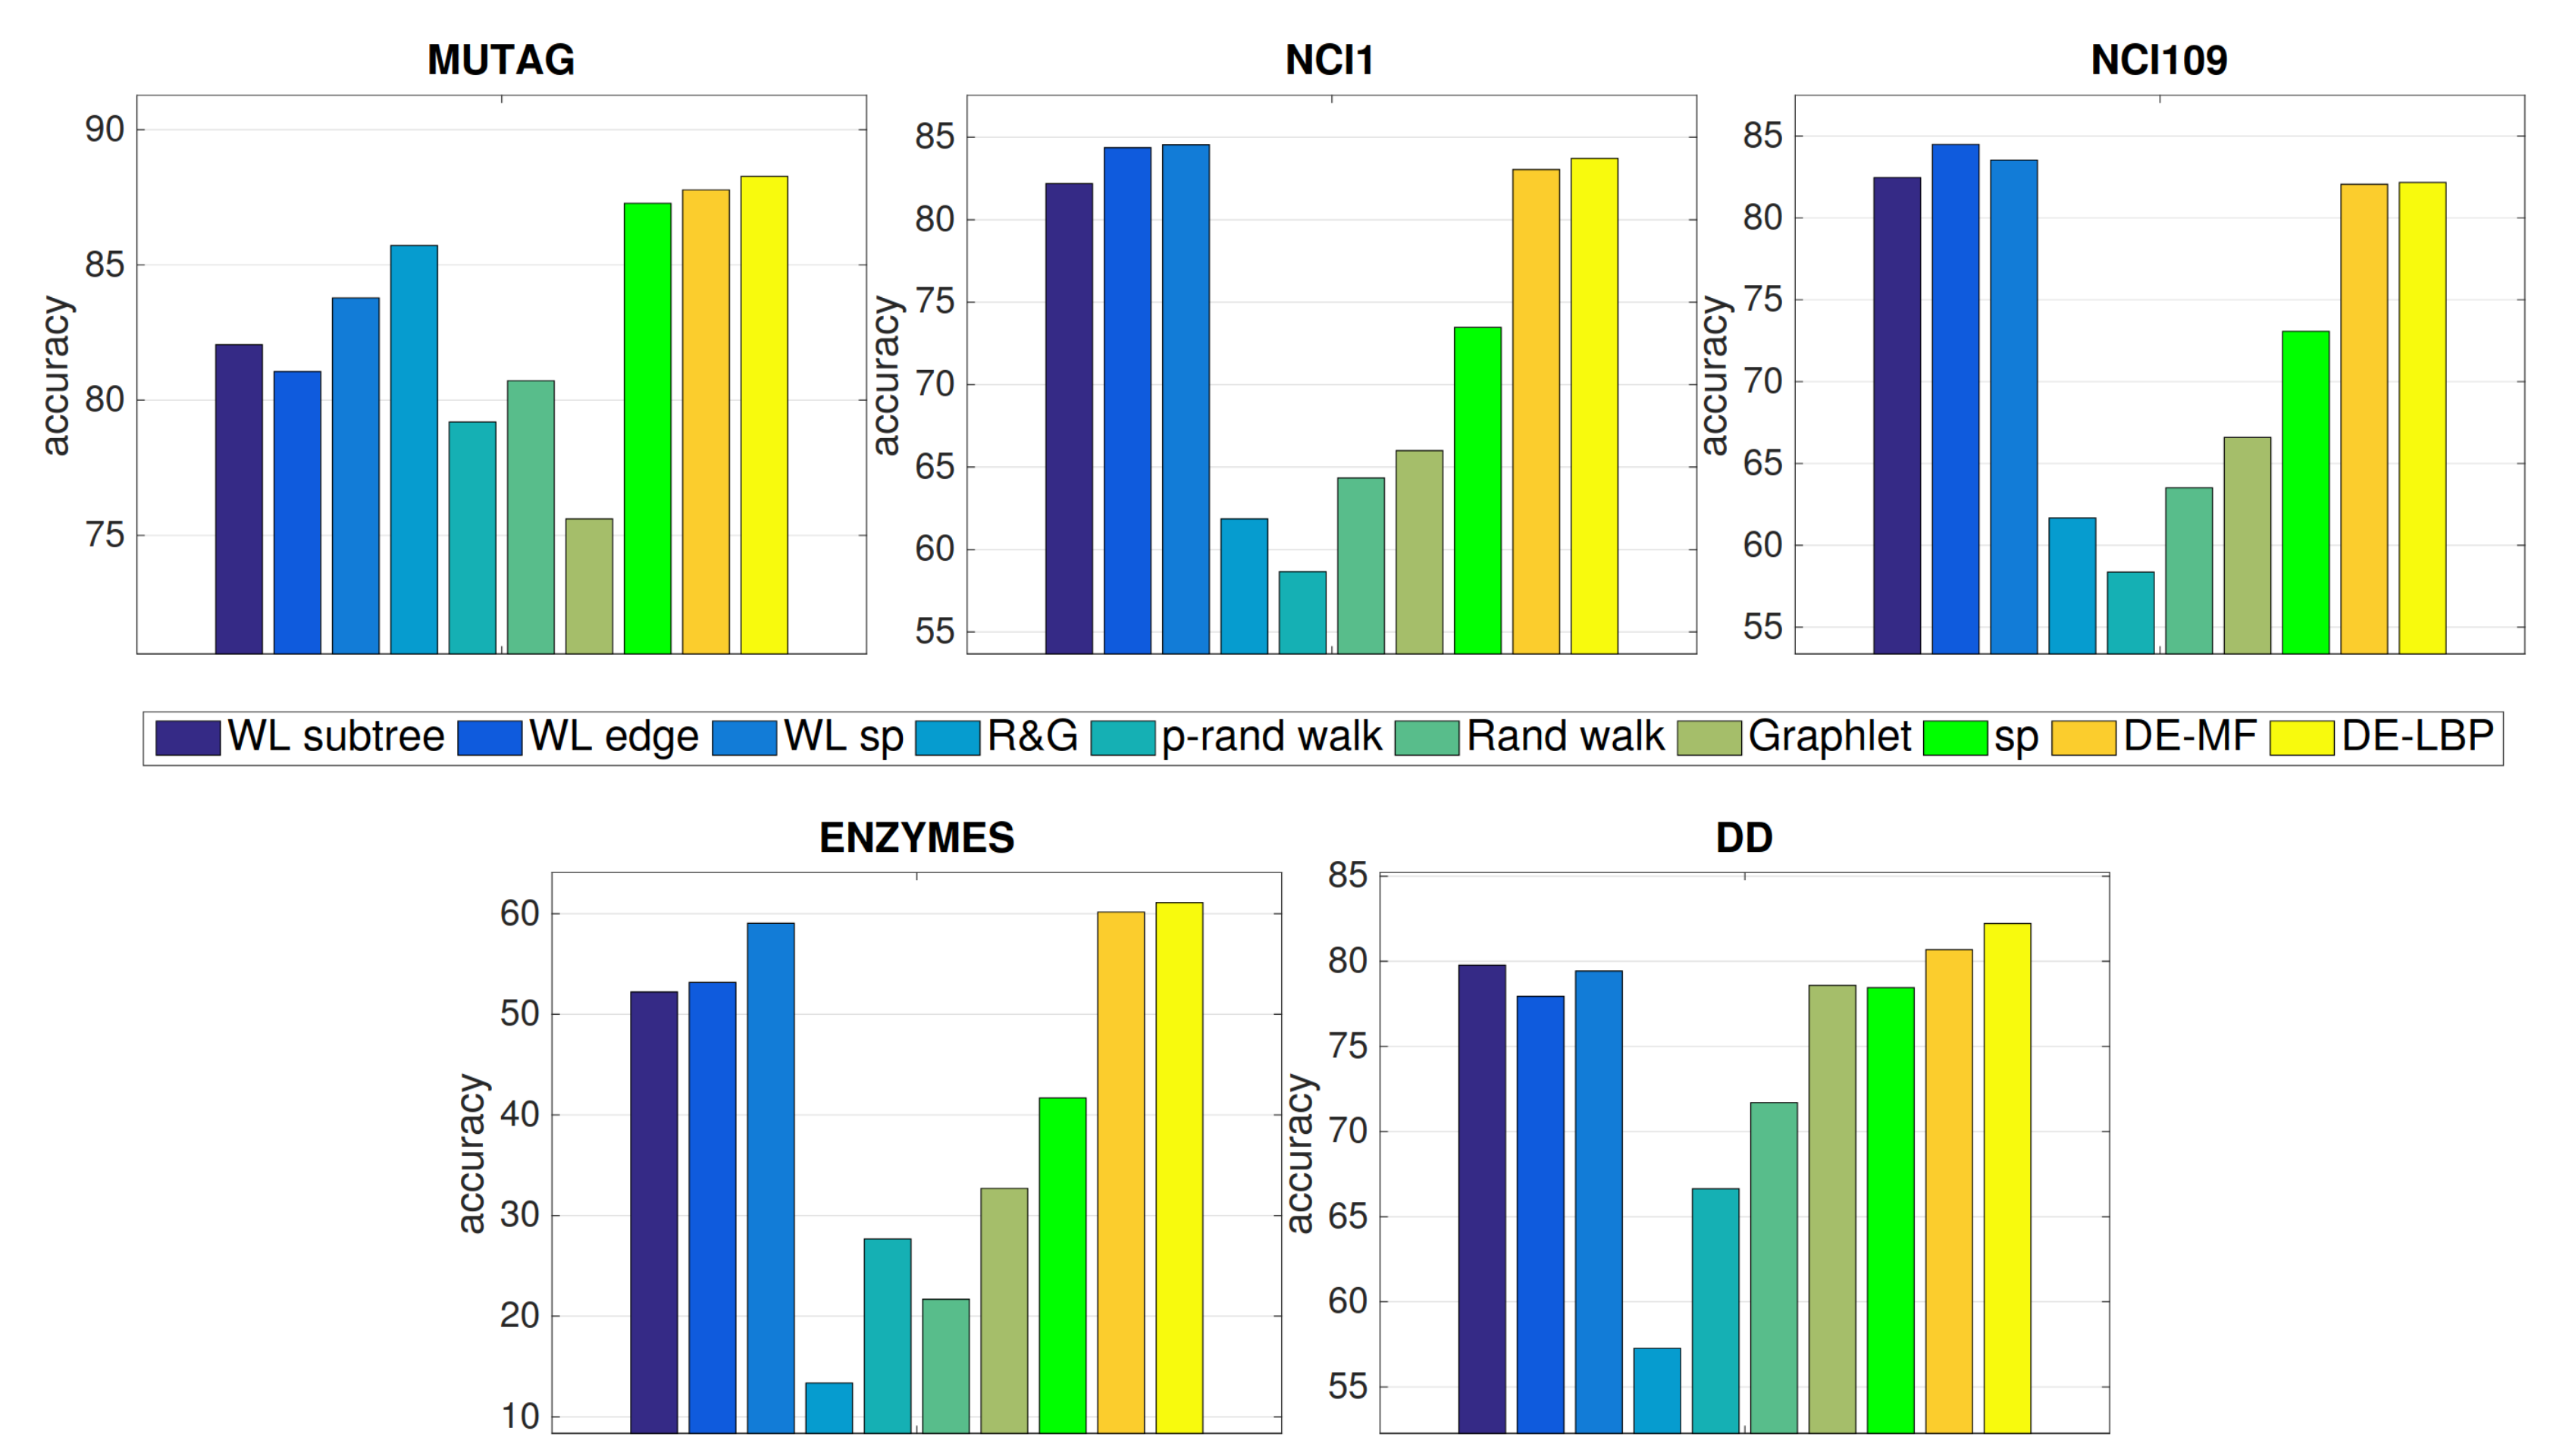
\includegraphics[width=\textwidth]{results.png}
        \end{center}
    \end{frame}

    \begin{frame}
        \frametitle{Resources}
        \begin{itemize}
            \item \href{https://people.eecs.berkeley.edu/~jordan/kernels/0521813972c03_p47-84.pdf}{Properties of kernels} \\
            \item \href{https://arxiv.org/pdf/1903.11835.pdf}{Survey on Graph Kernels} \\
            \item \href{https://www.cs.mcgill.ca/~prakash/Courses/599/Notes/metric_spaces.pdf}{Notes Metric Spaces}
        \end{itemize}
    \end{frame}
\end{document}